\section{Software Layers}

Die folgenden Diagramme beschreiben die Umsetzung zuerst Technologie-Unabhängig und danach mit der effektiven Implementation.\\
Durchgezogene Pfeile sind dabei als synchrone Kommunikation zu verstehen. Gestrichelte Pfeile als asynchrone Kommunikation.

\subsection*{Technologie-Unabhängig}

\begin{figure}[ht!]
	\centering{
		% Graphic for TeX using PGF
% Title: /Users/michael/code/BA/dokumentation/content/sad/layers-diagram.dia
% Creator: Dia v0.97.2
% CreationDate: Tue Mar 12 21:28:51 2013
% For: michael
% \usepackage{tikz}
% The following commands are not supported in PSTricks at present
% We define them conditionally, so when they are implemented,
% this pgf file will use them.
\ifx\du\undefined
  \newlength{\du}
\fi
\setlength{\du}{15\unitlength}
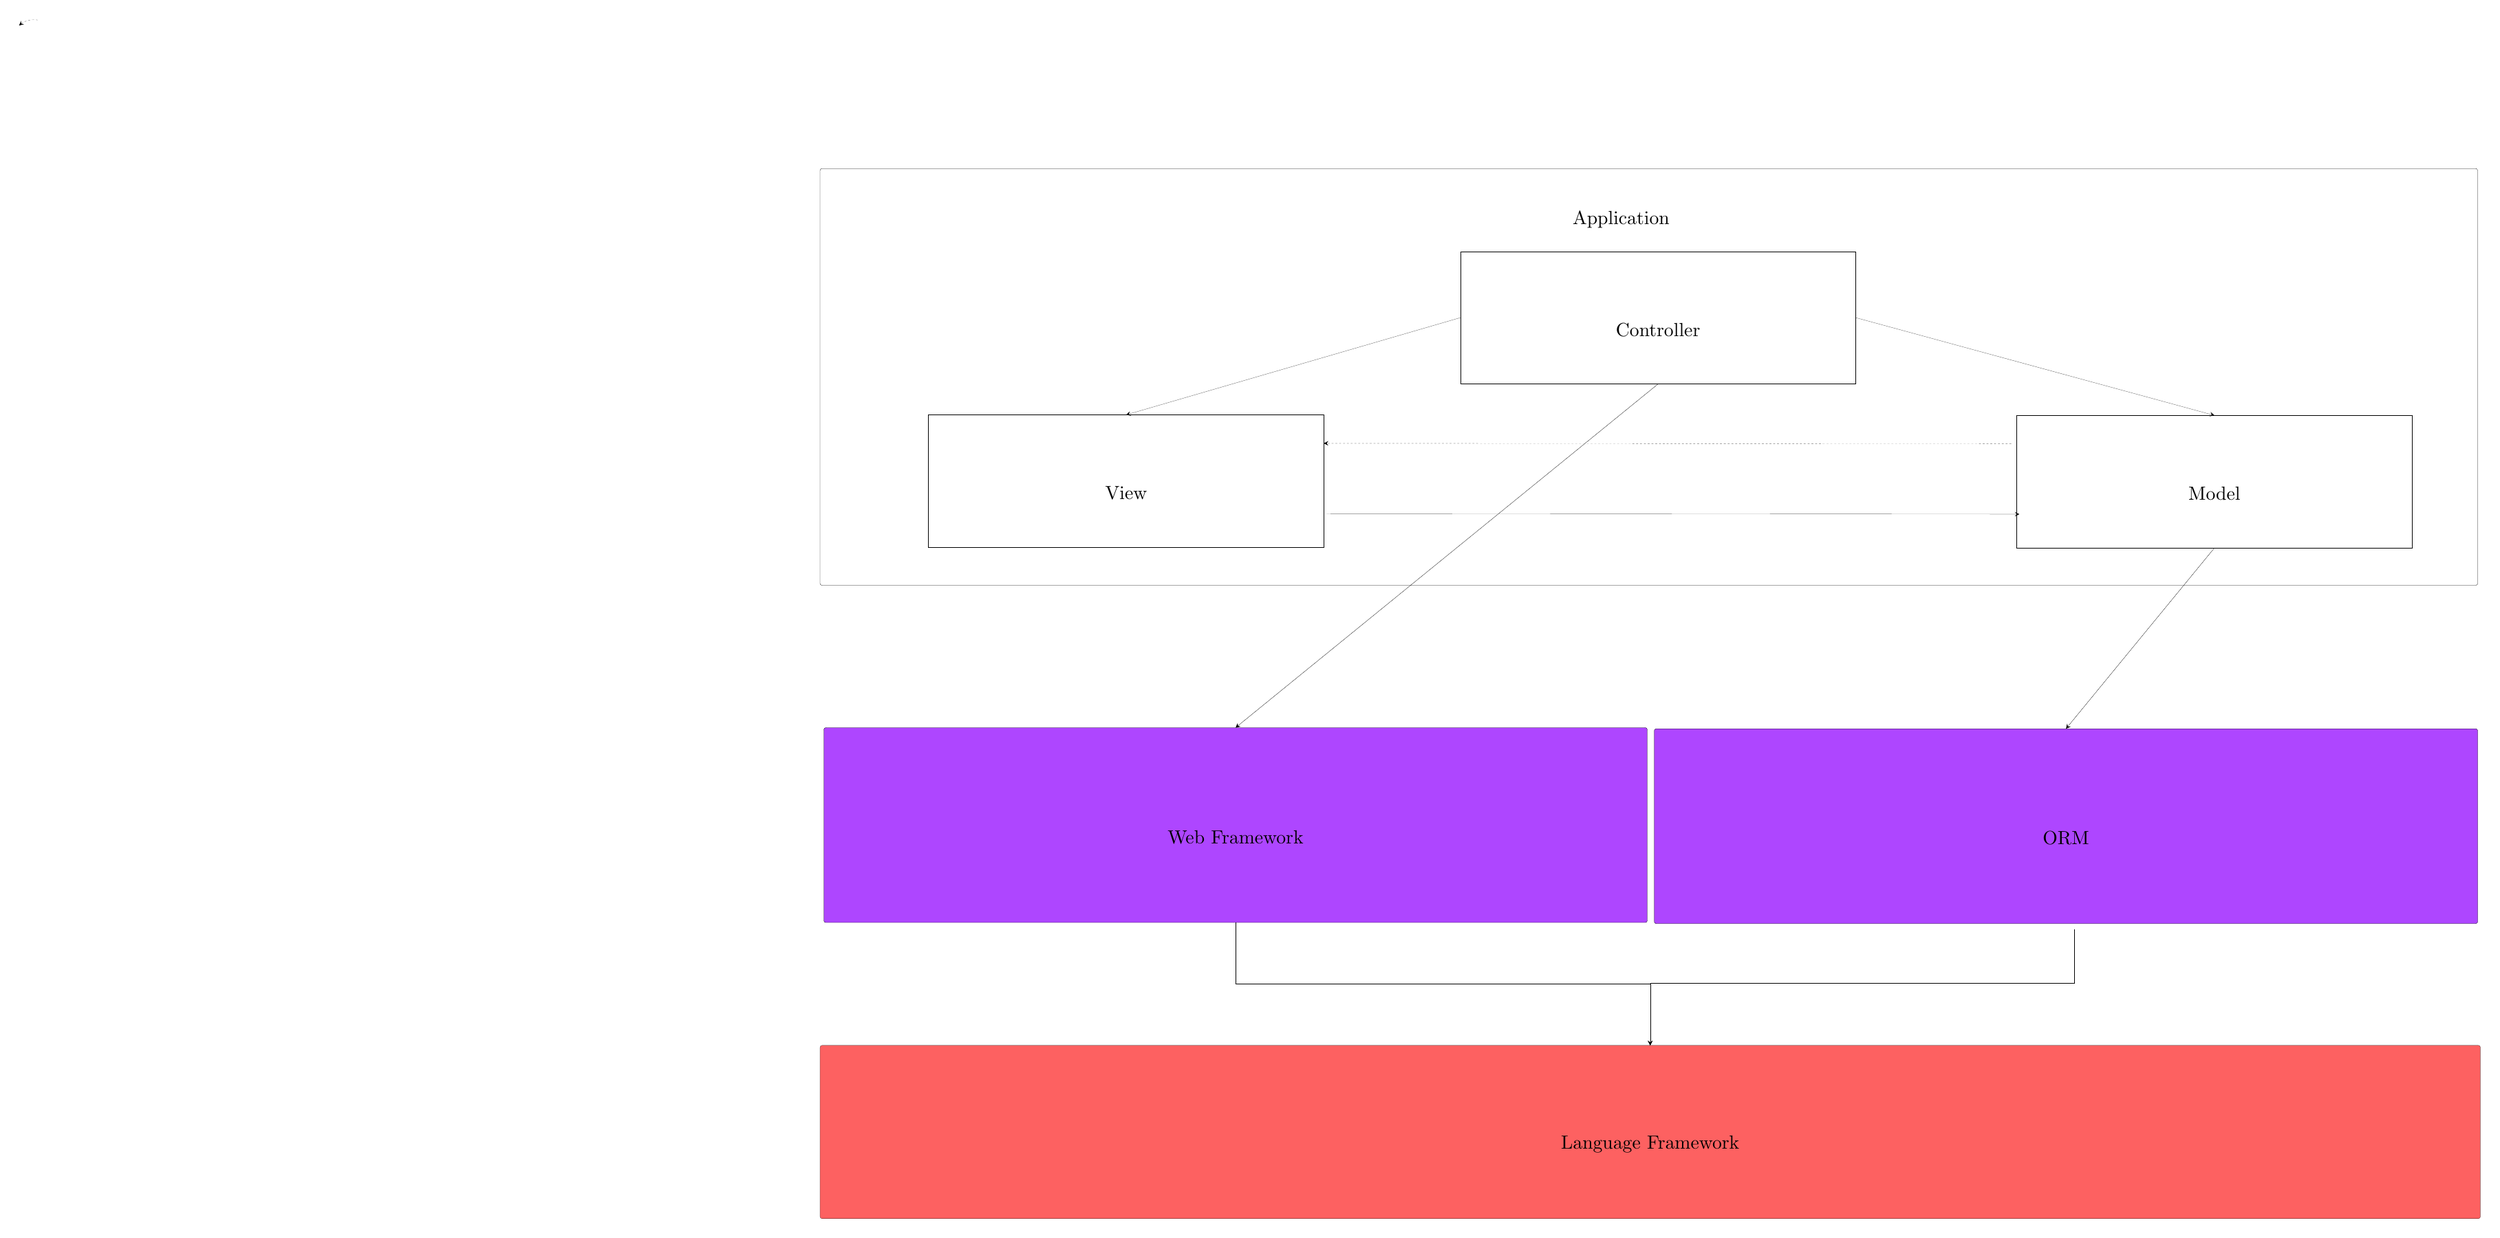
\begin{tikzpicture}
\pgftransformxscale{1.000000}
\pgftransformyscale{-1.000000}
\definecolor{dialinecolor}{rgb}{0.000000, 0.000000, 0.000000}
\pgfsetstrokecolor{dialinecolor}
\definecolor{dialinecolor}{rgb}{1.000000, 1.000000, 1.000000}
\pgfsetfillcolor{dialinecolor}
\pgfsetlinewidth{0.050000\du}
\pgfsetdash{}{0pt}
\pgfsetdash{}{0pt}
\pgfsetroundjoin
{\pgfsetcornersarced{\pgfpoint{1.000000\du}{1.000000\du}}\definecolor{dialinecolor}{rgb}{0.992157, 0.380392, 0.380392}
\pgfsetfillcolor{dialinecolor}
\fill (15.400000\du,19.100000\du)--(15.400000\du,22.300000\du)--(46.050000\du,22.300000\du)--(46.050000\du,19.100000\du)--cycle;
}{\pgfsetcornersarced{\pgfpoint{1.000000\du}{1.000000\du}}\definecolor{dialinecolor}{rgb}{0.000000, 0.000000, 0.000000}
\pgfsetstrokecolor{dialinecolor}
\draw (15.400000\du,19.100000\du)--(15.400000\du,22.300000\du)--(46.050000\du,22.300000\du)--(46.050000\du,19.100000\du)--cycle;
}% setfont left to latex
\definecolor{dialinecolor}{rgb}{0.000000, 0.000000, 0.000000}
\pgfsetstrokecolor{dialinecolor}
\node at (30.725000\du,20.922500\du){Language Framework};
\pgfsetlinewidth{0.100000\du}
\pgfsetdash{}{0pt}
\pgfsetdash{}{0pt}
\pgfsetroundjoin
{\pgfsetcornersarced{\pgfpoint{1.000000\du}{1.000000\du}}\definecolor{dialinecolor}{rgb}{1.000000, 1.000000, 1.000000}
\pgfsetfillcolor{dialinecolor}
\fill (15.400000\du,2.900000\du)--(15.400000\du,10.600000\du)--(46.000000\du,10.600000\du)--(46.000000\du,2.900000\du)--cycle;
}{\pgfsetcornersarced{\pgfpoint{1.000000\du}{1.000000\du}}\definecolor{dialinecolor}{rgb}{0.000000, 0.000000, 0.000000}
\pgfsetstrokecolor{dialinecolor}
\draw (15.400000\du,2.900000\du)--(15.400000\du,10.600000\du)--(46.000000\du,10.600000\du)--(46.000000\du,2.900000\du)--cycle;
}% setfont left to latex
\definecolor{dialinecolor}{rgb}{0.000000, 0.000000, 0.000000}
\pgfsetstrokecolor{dialinecolor}
\node[anchor=west] at (29.175000\du,3.850000\du){Application};
\pgfsetlinewidth{0.100000\du}
\pgfsetdash{}{0pt}
\pgfsetdash{}{0pt}
\pgfsetmiterjoin
\definecolor{dialinecolor}{rgb}{1.000000, 1.000000, 1.000000}
\pgfsetfillcolor{dialinecolor}
\fill (17.400000\du,7.450000\du)--(17.400000\du,9.900000\du)--(24.700000\du,9.900000\du)--(24.700000\du,7.450000\du)--cycle;
\definecolor{dialinecolor}{rgb}{0.000000, 0.000000, 0.000000}
\pgfsetstrokecolor{dialinecolor}
\draw (17.400000\du,7.450000\du)--(17.400000\du,9.900000\du)--(24.700000\du,9.900000\du)--(24.700000\du,7.450000\du)--cycle;
% setfont left to latex
\definecolor{dialinecolor}{rgb}{0.000000, 0.000000, 0.000000}
\pgfsetstrokecolor{dialinecolor}
\node at (21.050000\du,8.897500\du){View};
\pgfsetlinewidth{0.100000\du}
\pgfsetdash{}{0pt}
\pgfsetdash{}{0pt}
\pgfsetroundjoin
{\pgfsetcornersarced{\pgfpoint{1.000000\du}{1.000000\du}}\definecolor{dialinecolor}{rgb}{0.682353, 0.274510, 1.000000}
\pgfsetfillcolor{dialinecolor}
\fill (30.800000\du,13.250000\du)--(30.800000\du,16.850000\du)--(46.000000\du,16.850000\du)--(46.000000\du,13.250000\du)--cycle;
}{\pgfsetcornersarced{\pgfpoint{1.000000\du}{1.000000\du}}\definecolor{dialinecolor}{rgb}{0.000000, 0.000000, 0.000000}
\pgfsetstrokecolor{dialinecolor}
\draw (30.800000\du,13.250000\du)--(30.800000\du,16.850000\du)--(46.000000\du,16.850000\du)--(46.000000\du,13.250000\du)--cycle;
}% setfont left to latex
\definecolor{dialinecolor}{rgb}{0.000000, 0.000000, 0.000000}
\pgfsetstrokecolor{dialinecolor}
\node at (38.400000\du,15.272500\du){ORM};
\pgfsetlinewidth{0.100000\du}
\pgfsetdash{}{0pt}
\pgfsetdash{}{0pt}
\pgfsetroundjoin
{\pgfsetcornersarced{\pgfpoint{1.000000\du}{1.000000\du}}\definecolor{dialinecolor}{rgb}{0.682353, 0.274510, 1.000000}
\pgfsetfillcolor{dialinecolor}
\fill (15.470000\du,13.230000\du)--(15.470000\du,16.830000\du)--(30.670000\du,16.830000\du)--(30.670000\du,13.230000\du)--cycle;
}{\pgfsetcornersarced{\pgfpoint{1.000000\du}{1.000000\du}}\definecolor{dialinecolor}{rgb}{0.000000, 0.000000, 0.000000}
\pgfsetstrokecolor{dialinecolor}
\draw (15.470000\du,13.230000\du)--(15.470000\du,16.830000\du)--(30.670000\du,16.830000\du)--(30.670000\du,13.230000\du)--cycle;
}% setfont left to latex
\definecolor{dialinecolor}{rgb}{0.000000, 0.000000, 0.000000}
\pgfsetstrokecolor{dialinecolor}
\node at (23.070000\du,15.252500\du){Web Framework};
\pgfsetlinewidth{0.100000\du}
\pgfsetdash{}{0pt}
\pgfsetdash{}{0pt}
\pgfsetmiterjoin
\definecolor{dialinecolor}{rgb}{1.000000, 1.000000, 1.000000}
\pgfsetfillcolor{dialinecolor}
\fill (27.220000\du,4.430000\du)--(27.220000\du,6.880000\du)--(34.520000\du,6.880000\du)--(34.520000\du,4.430000\du)--cycle;
\definecolor{dialinecolor}{rgb}{0.000000, 0.000000, 0.000000}
\pgfsetstrokecolor{dialinecolor}
\draw (27.220000\du,4.430000\du)--(27.220000\du,6.880000\du)--(34.520000\du,6.880000\du)--(34.520000\du,4.430000\du)--cycle;
\pgfsetlinewidth{0.100000\du}
\pgfsetdash{}{0pt}
\pgfsetdash{}{0pt}
\pgfsetmiterjoin
\definecolor{dialinecolor}{rgb}{1.000000, 1.000000, 1.000000}
\pgfsetfillcolor{dialinecolor}
\fill (37.490000\du,7.460000\du)--(37.490000\du,9.910000\du)--(44.790000\du,9.910000\du)--(44.790000\du,7.460000\du)--cycle;
\definecolor{dialinecolor}{rgb}{0.000000, 0.000000, 0.000000}
\pgfsetstrokecolor{dialinecolor}
\draw (37.490000\du,7.460000\du)--(37.490000\du,9.910000\du)--(44.790000\du,9.910000\du)--(44.790000\du,7.460000\du)--cycle;
% setfont left to latex
\definecolor{dialinecolor}{rgb}{0.000000, 0.000000, 0.000000}
\pgfsetstrokecolor{dialinecolor}
\node at (30.870000\du,5.877500\du){Controller};
% setfont left to latex
\definecolor{dialinecolor}{rgb}{0.000000, 0.000000, 0.000000}
\pgfsetstrokecolor{dialinecolor}
\node at (41.140000\du,8.907500\du){Model};
\pgfsetlinewidth{0.050000\du}
\pgfsetdash{}{0pt}
\pgfsetdash{}{0pt}
\pgfsetbuttcap
{
\definecolor{dialinecolor}{rgb}{0.000000, 0.000000, 0.000000}
\pgfsetfillcolor{dialinecolor}
% was here!!!
\pgfsetarrowsend{stealth}
\definecolor{dialinecolor}{rgb}{0.000000, 0.000000, 0.000000}
\pgfsetstrokecolor{dialinecolor}
\draw (27.220000\du,5.655000\du)--(21.050000\du,7.450000\du);
}
\pgfsetlinewidth{0.050000\du}
\pgfsetdash{}{0pt}
\pgfsetdash{}{0pt}
\pgfsetbuttcap
{
\definecolor{dialinecolor}{rgb}{0.000000, 0.000000, 0.000000}
\pgfsetfillcolor{dialinecolor}
% was here!!!
\pgfsetarrowsend{stealth}
\definecolor{dialinecolor}{rgb}{0.000000, 0.000000, 0.000000}
\pgfsetstrokecolor{dialinecolor}
\draw (34.520000\du,5.655000\du)--(41.140000\du,7.460000\du);
}
\pgfsetlinewidth{0.050000\du}
\pgfsetdash{}{0pt}
\pgfsetdash{}{0pt}
\pgfsetbuttcap
{
\definecolor{dialinecolor}{rgb}{0.000000, 0.000000, 0.000000}
\pgfsetfillcolor{dialinecolor}
% was here!!!
\pgfsetarrowsend{stealth}
\definecolor{dialinecolor}{rgb}{0.000000, 0.000000, 0.000000}
\pgfsetstrokecolor{dialinecolor}
\draw (24.750000\du,9.275000\du)--(37.540000\du,9.285000\du);
}
\pgfsetlinewidth{0.050000\du}
\pgfsetdash{{1.000000\du}{1.000000\du}}{0\du}
\pgfsetdash{{1.000000\du}{1.000000\du}}{0\du}
\pgfsetbuttcap
{
\definecolor{dialinecolor}{rgb}{0.000000, 0.000000, 0.000000}
\pgfsetfillcolor{dialinecolor}
% was here!!!
\pgfsetarrowsend{stealth}
\definecolor{dialinecolor}{rgb}{0.000000, 0.000000, 0.000000}
\pgfsetstrokecolor{dialinecolor}
\draw (37.390600\du,7.983160\du)--(24.699400\du,7.976840\du);
}
\pgfsetlinewidth{0.100000\du}
\pgfsetdash{}{0pt}
\pgfsetdash{}{0pt}
\pgfsetbuttcap
{
\definecolor{dialinecolor}{rgb}{0.000000, 0.000000, 0.000000}
\pgfsetfillcolor{dialinecolor}
% was here!!!
\pgfsetarrowsend{stealth}
\definecolor{dialinecolor}{rgb}{0.000000, 0.000000, 0.000000}
\pgfsetstrokecolor{dialinecolor}
\draw (30.870000\du,6.880000\du)--(23.070000\du,13.230000\du);
}
\pgfsetlinewidth{0.100000\du}
\pgfsetdash{}{0pt}
\pgfsetdash{}{0pt}
\pgfsetbuttcap
{
\definecolor{dialinecolor}{rgb}{0.000000, 0.000000, 0.000000}
\pgfsetfillcolor{dialinecolor}
% was here!!!
\pgfsetarrowsend{stealth}
\definecolor{dialinecolor}{rgb}{0.000000, 0.000000, 0.000000}
\pgfsetstrokecolor{dialinecolor}
\draw (41.140000\du,9.910000\du)--(38.400000\du,13.250000\du);
}
\pgfsetlinewidth{0.100000\du}
\pgfsetdash{}{0pt}
\pgfsetdash{}{0pt}
\pgfsetmiterjoin
\pgfsetbuttcap
{
\definecolor{dialinecolor}{rgb}{0.000000, 0.000000, 0.000000}
\pgfsetfillcolor{dialinecolor}
% was here!!!
\pgfsetarrowsend{stealth}
{\pgfsetcornersarced{\pgfpoint{0.000000\du}{0.000000\du}}\definecolor{dialinecolor}{rgb}{0.000000, 0.000000, 0.000000}
\pgfsetstrokecolor{dialinecolor}
\draw (23.070000\du,16.830000\du)--(23.070000\du,17.965000\du)--(30.725000\du,17.965000\du)--(30.725000\du,19.100000\du);
}}
\pgfsetlinewidth{0.100000\du}
\pgfsetdash{}{0pt}
\pgfsetdash{}{0pt}
\pgfsetmiterjoin
\pgfsetbuttcap
{
\definecolor{dialinecolor}{rgb}{0.000000, 0.000000, 0.000000}
\pgfsetfillcolor{dialinecolor}
% was here!!!
\pgfsetarrowsend{stealth}
{\pgfsetcornersarced{\pgfpoint{0.000000\du}{0.000000\du}}\definecolor{dialinecolor}{rgb}{0.000000, 0.000000, 0.000000}
\pgfsetstrokecolor{dialinecolor}
\draw (38.550000\du,16.950000\du)--(38.550000\du,17.950000\du)--(30.725000\du,17.950000\du)--(30.725000\du,19.100000\du);
}}
\pgfsetlinewidth{0.050000\du}
\pgfsetdash{{1.000000\du}{1.000000\du}}{0\du}
\pgfsetdash{{1.000000\du}{1.000000\du}}{0\du}
\pgfsetbuttcap
{
\definecolor{dialinecolor}{rgb}{0.000000, 0.000000, 0.000000}
\pgfsetfillcolor{dialinecolor}
% was here!!!
\pgfsetarrowsend{stealth}
\definecolor{dialinecolor}{rgb}{0.000000, 0.000000, 0.000000}
\pgfsetstrokecolor{dialinecolor}
\pgfpathmoveto{\pgfpoint{27.220293\du}{4.430039\du}}
\pgfpatharc{278}{229}{12.284917\du and 12.284917\du}
\pgfusepath{stroke}
}
\end{tikzpicture}

	}

	\caption{Software Layers -- Technologie-Unabhängig}
\end{figure}

\subsubsection*{Client-Side}
Diese Schicht wird im Browser selber als JavaScript ausgeführt und synchronisiert sich mit dem Server über URLs.

\subsubsection*{Business}
In der Business-Schicht wird die eigentliche Business-Logik definiert und mit der Datenbank über Models kommuniziert.

\subsubsection*{Language Framework}
Das Language Framework wird von \gls{nodejs} zur Verfügung gestellt.

\subsubsection*{Security}
Sowohl Client wie auch Server beinhalten einige Sicherheitsmassnahmen um zu gewährleisten, dass ein \gls{Bewohner} immer authentisiert ist und keine gefährlichen Daten übermitteln kann.

\newpage
\subsection*{Implementation}

\begin{figure}[ht!]
	\centering{
		% Graphic for TeX using PGF
% Title: /Users/michael/code/BA/dokumentation/content/sad/layers-diagram-impl.dia
% Creator: Dia v0.97.2
% CreationDate: Tue Mar 12 22:27:26 2013
% For: michael
% \usepackage{tikz}
% The following commands are not supported in PSTricks at present
% We define them conditionally, so when they are implemented,
% this pgf file will use them.
\ifx\du\undefined
  \newlength{\du}
\fi
\setlength{\du}{15\unitlength}
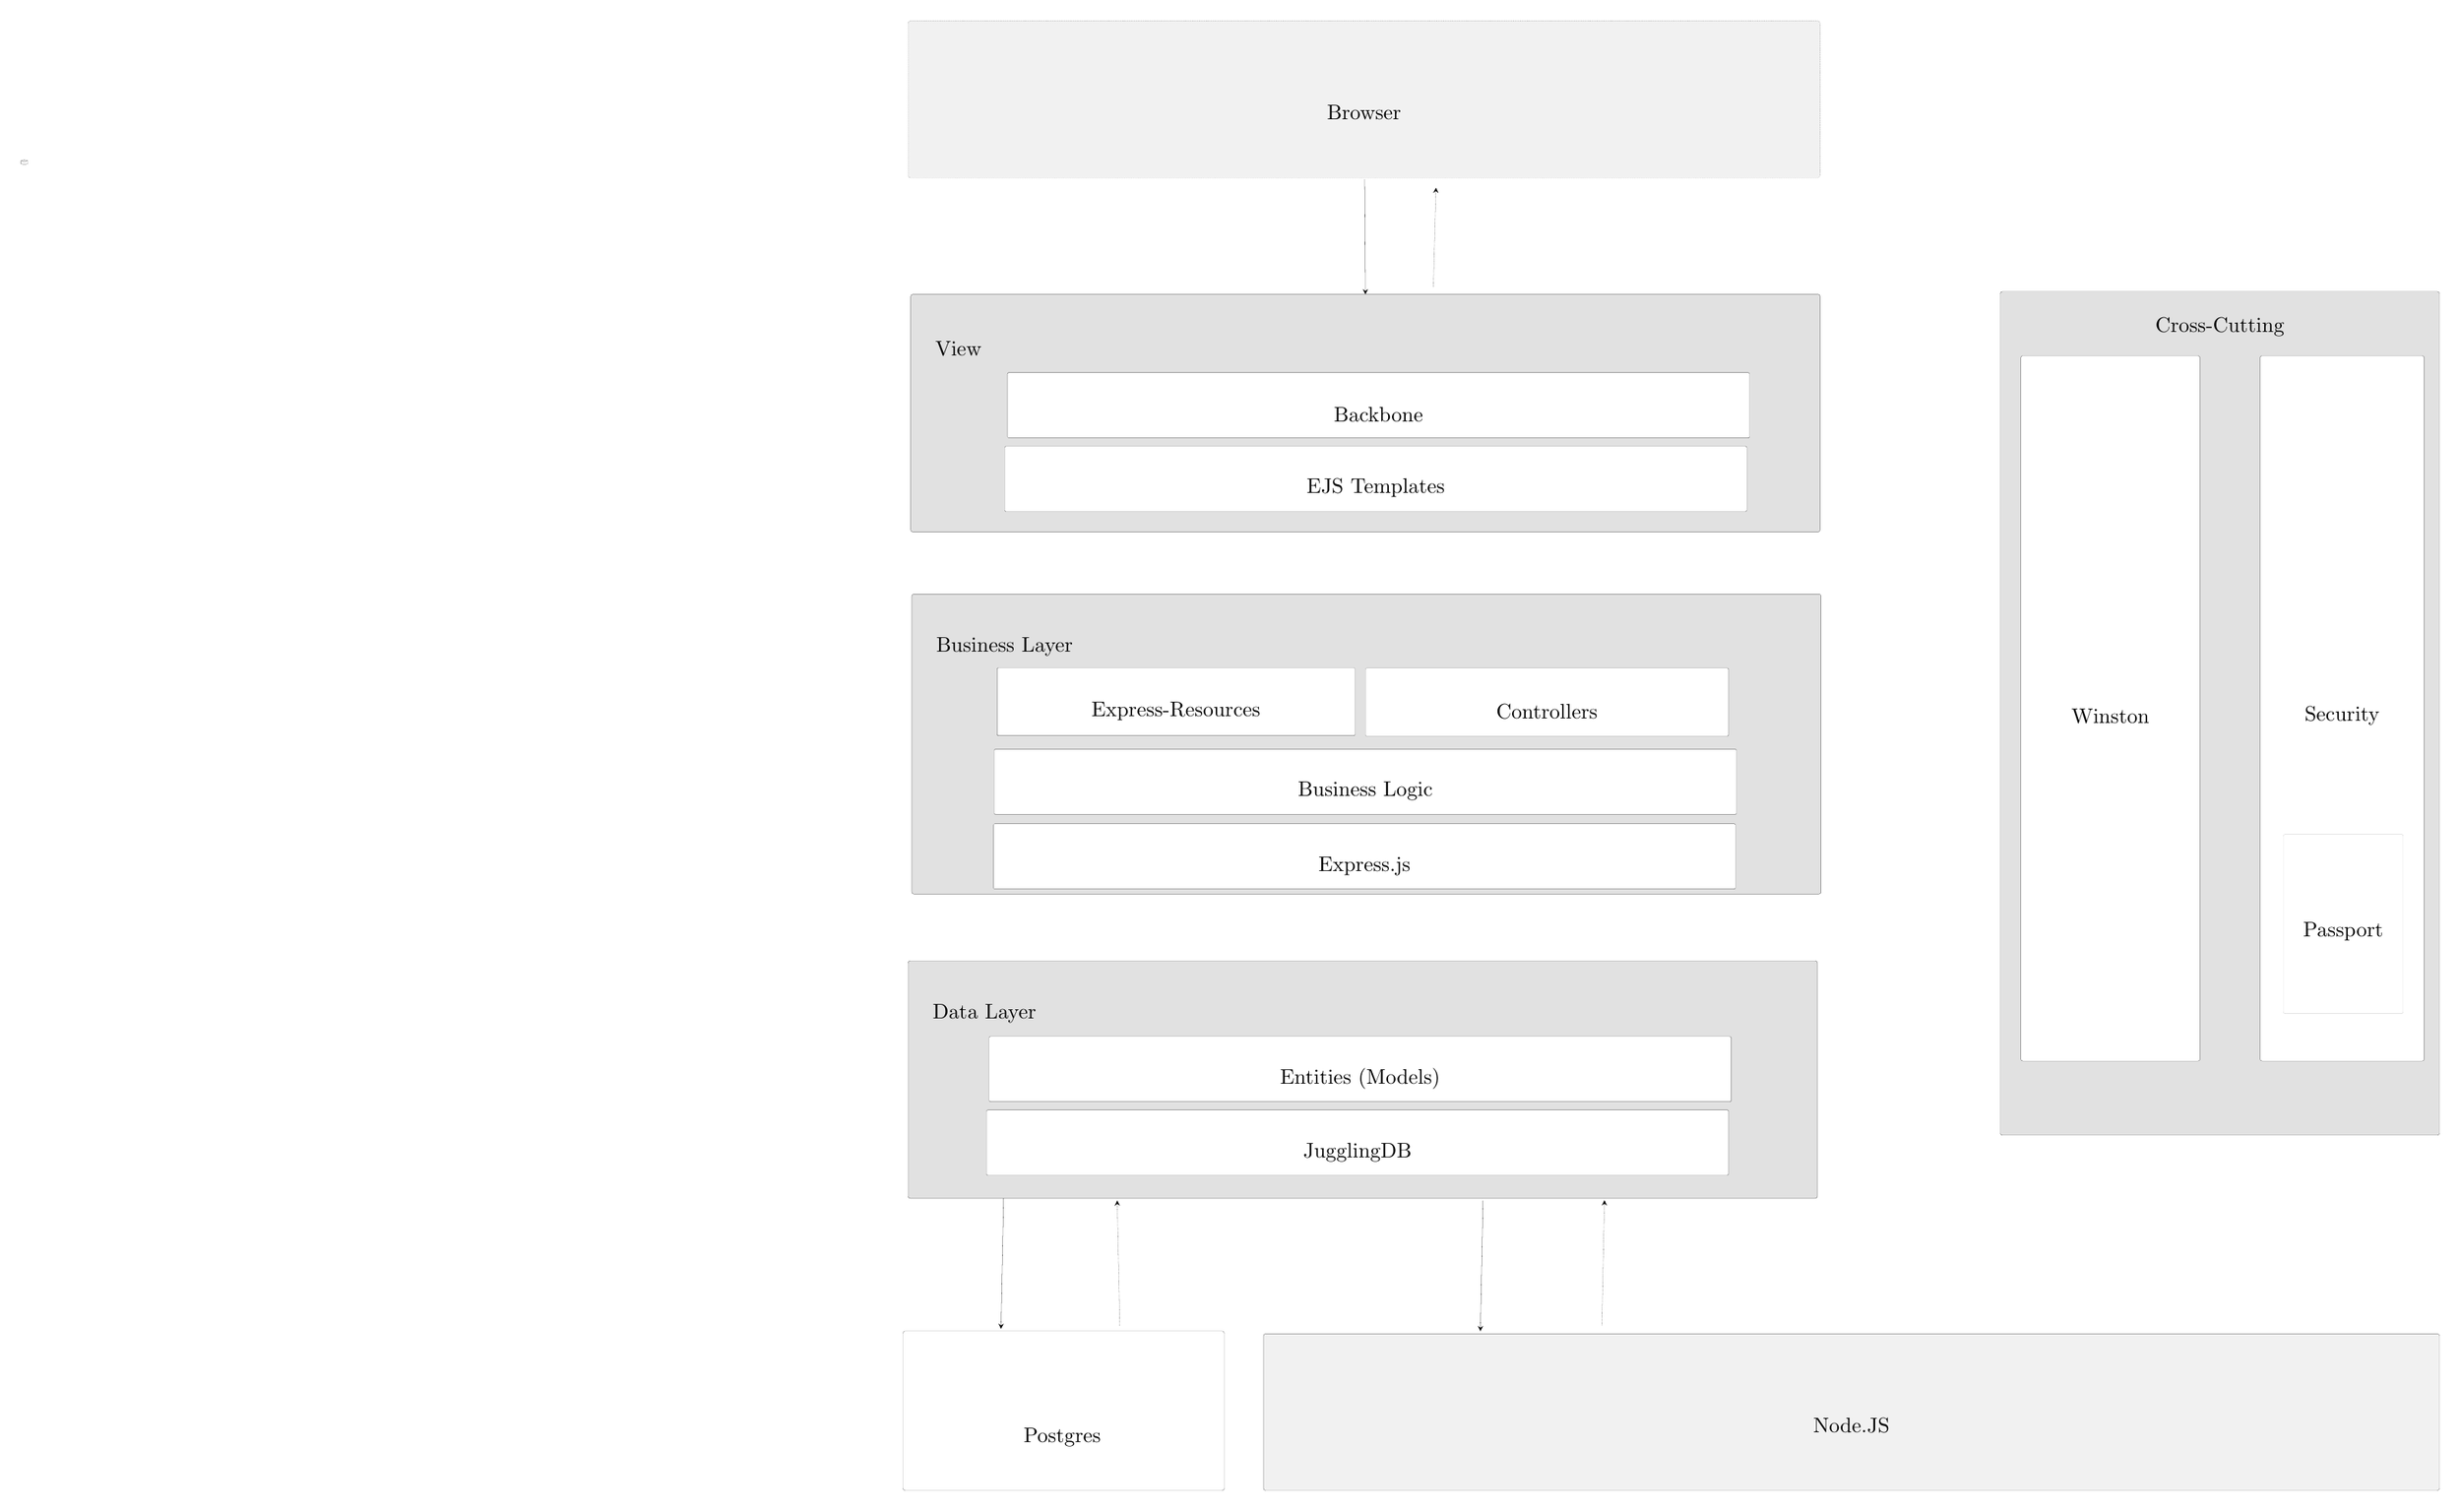
\begin{tikzpicture}
\pgftransformxscale{1.000000}
\pgftransformyscale{-1.000000}
\definecolor{dialinecolor}{rgb}{0.000000, 0.000000, 0.000000}
\pgfsetstrokecolor{dialinecolor}
\definecolor{dialinecolor}{rgb}{1.000000, 1.000000, 1.000000}
\pgfsetfillcolor{dialinecolor}
\pgfsetlinewidth{0.050000\du}
\pgfsetdash{}{0pt}
\pgfsetdash{}{0pt}
\pgfsetroundjoin
{\pgfsetcornersarced{\pgfpoint{1.000000\du}{1.000000\du}}\definecolor{dialinecolor}{rgb}{0.882353, 0.882353, 0.882353}
\pgfsetfillcolor{dialinecolor}
\fill (33.658750\du,2.925000\du)--(33.658750\du,17.034356\du)--(41.000000\du,17.034356\du)--(41.000000\du,2.925000\du)--cycle;
}{\pgfsetcornersarced{\pgfpoint{1.000000\du}{1.000000\du}}\definecolor{dialinecolor}{rgb}{0.000000, 0.000000, 0.000000}
\pgfsetstrokecolor{dialinecolor}
\draw (33.658750\du,2.925000\du)--(33.658750\du,17.034356\du)--(41.000000\du,17.034356\du)--(41.000000\du,2.925000\du)--cycle;
}% setfont left to latex
\definecolor{dialinecolor}{rgb}{0.000000, 0.000000, 0.000000}
\pgfsetstrokecolor{dialinecolor}
\node[anchor=west] at (37.329375\du,9.979678\du){};
% setfont left to latex
\definecolor{dialinecolor}{rgb}{0.000000, 0.000000, 0.000000}
\pgfsetstrokecolor{dialinecolor}
\node at (37.329375\du,3.520000\du){Cross-Cutting};
\pgfsetlinewidth{0.050000\du}
\pgfsetdash{}{0pt}
\pgfsetdash{}{0pt}
\pgfsetroundjoin
{\pgfsetcornersarced{\pgfpoint{1.000000\du}{1.000000\du}}\definecolor{dialinecolor}{rgb}{0.882353, 0.882353, 0.882353}
\pgfsetfillcolor{dialinecolor}
\fill (15.448447\du,2.971250\du)--(15.448447\du,6.945606\du)--(30.647083\du,6.945606\du)--(30.647083\du,2.971250\du)--cycle;
}{\pgfsetcornersarced{\pgfpoint{1.000000\du}{1.000000\du}}\definecolor{dialinecolor}{rgb}{0.000000, 0.000000, 0.000000}
\pgfsetstrokecolor{dialinecolor}
\draw (15.448447\du,2.971250\du)--(15.448447\du,6.945606\du)--(30.647083\du,6.945606\du)--(30.647083\du,2.971250\du)--cycle;
}\pgfsetlinewidth{0.050000\du}
\pgfsetdash{}{0pt}
\pgfsetdash{}{0pt}
\pgfsetroundjoin
{\pgfsetcornersarced{\pgfpoint{1.000000\du}{1.000000\du}}\definecolor{dialinecolor}{rgb}{0.882353, 0.882353, 0.882353}
\pgfsetfillcolor{dialinecolor}
\fill (15.403568\du,14.115712\du)--(15.403568\du,18.090068\du)--(30.602205\du,18.090068\du)--(30.602205\du,14.115712\du)--cycle;
}{\pgfsetcornersarced{\pgfpoint{1.000000\du}{1.000000\du}}\definecolor{dialinecolor}{rgb}{0.000000, 0.000000, 0.000000}
\pgfsetstrokecolor{dialinecolor}
\draw (15.403568\du,14.115712\du)--(15.403568\du,18.090068\du)--(30.602205\du,18.090068\du)--(30.602205\du,14.115712\du)--cycle;
}\pgfsetlinewidth{0.050000\du}
\pgfsetdash{}{0pt}
\pgfsetdash{}{0pt}
\pgfsetroundjoin
{\pgfsetcornersarced{\pgfpoint{1.000000\du}{1.000000\du}}\definecolor{dialinecolor}{rgb}{0.882353, 0.882353, 0.882353}
\pgfsetfillcolor{dialinecolor}
\fill (15.464712\du,7.983848\du)--(15.464712\du,13.000000\du)--(30.663348\du,13.000000\du)--(30.663348\du,7.983848\du)--cycle;
}{\pgfsetcornersarced{\pgfpoint{1.000000\du}{1.000000\du}}\definecolor{dialinecolor}{rgb}{0.000000, 0.000000, 0.000000}
\pgfsetstrokecolor{dialinecolor}
\draw (15.464712\du,7.983848\du)--(15.464712\du,13.000000\du)--(30.663348\du,13.000000\du)--(30.663348\du,7.983848\du)--cycle;
}% setfont left to latex
\definecolor{dialinecolor}{rgb}{0.000000, 0.000000, 0.000000}
\pgfsetstrokecolor{dialinecolor}
\node[anchor=west] at (15.741340\du,3.877768\du){View};
% setfont left to latex
\definecolor{dialinecolor}{rgb}{0.000000, 0.000000, 0.000000}
\pgfsetstrokecolor{dialinecolor}
\node[anchor=west] at (15.757605\du,8.871742\du){Business Layer};
% setfont left to latex
\definecolor{dialinecolor}{rgb}{0.000000, 0.000000, 0.000000}
\pgfsetstrokecolor{dialinecolor}
\node[anchor=west] at (15.696461\du,15.003605\du){Data Layer};
\pgfsetlinewidth{0.050000\du}
\pgfsetdash{}{0pt}
\pgfsetdash{}{0pt}
\pgfsetroundjoin
{\pgfsetcornersarced{\pgfpoint{1.000000\du}{1.000000\du}}\definecolor{dialinecolor}{rgb}{0.945098, 0.945098, 0.945098}
\pgfsetfillcolor{dialinecolor}
\fill (21.344470\du,20.353598\du)--(21.344470\du,22.974053\du)--(41.000000\du,22.974053\du)--(41.000000\du,20.353598\du)--cycle;
}{\pgfsetcornersarced{\pgfpoint{1.000000\du}{1.000000\du}}\definecolor{dialinecolor}{rgb}{0.000000, 0.000000, 0.000000}
\pgfsetstrokecolor{dialinecolor}
\draw (21.344470\du,20.353598\du)--(21.344470\du,22.974053\du)--(41.000000\du,22.974053\du)--(41.000000\du,20.353598\du)--cycle;
}% setfont left to latex
\definecolor{dialinecolor}{rgb}{0.000000, 0.000000, 0.000000}
\pgfsetstrokecolor{dialinecolor}
\node at (31.172235\du,21.886326\du){Node.JS};
\pgfsetlinewidth{0.050000\du}
\pgfsetdash{}{0pt}
\pgfsetdash{}{0pt}
\pgfsetroundjoin
{\pgfsetcornersarced{\pgfpoint{0.500000\du}{0.500000\du}}\definecolor{dialinecolor}{rgb}{1.000000, 1.000000, 1.000000}
\pgfsetfillcolor{dialinecolor}
\fill (17.064394\du,4.281477\du)--(17.064394\du,5.373333\du)--(29.467879\du,5.373333\du)--(29.467879\du,4.281477\du)--cycle;
}{\pgfsetcornersarced{\pgfpoint{0.500000\du}{0.500000\du}}\definecolor{dialinecolor}{rgb}{0.000000, 0.000000, 0.000000}
\pgfsetstrokecolor{dialinecolor}
\draw (17.064394\du,4.281477\du)--(17.064394\du,5.373333\du)--(29.467879\du,5.373333\du)--(29.467879\du,4.281477\du)--cycle;
}\pgfsetlinewidth{0.050000\du}
\pgfsetdash{}{0pt}
\pgfsetdash{}{0pt}
\pgfsetroundjoin
{\pgfsetcornersarced{\pgfpoint{0.500000\du}{0.500000\du}}\definecolor{dialinecolor}{rgb}{1.000000, 1.000000, 1.000000}
\pgfsetfillcolor{dialinecolor}
\fill (17.019515\du,5.511886\du)--(17.019515\du,6.603742\du)--(29.423000\du,6.603742\du)--(29.423000\du,5.511886\du)--cycle;
}{\pgfsetcornersarced{\pgfpoint{0.500000\du}{0.500000\du}}\definecolor{dialinecolor}{rgb}{0.000000, 0.000000, 0.000000}
\pgfsetstrokecolor{dialinecolor}
\draw (17.019515\du,5.511886\du)--(17.019515\du,6.603742\du)--(29.423000\du,6.603742\du)--(29.423000\du,5.511886\du)--cycle;
}% setfont left to latex
\definecolor{dialinecolor}{rgb}{0.000000, 0.000000, 0.000000}
\pgfsetstrokecolor{dialinecolor}
\node at (23.266136\du,4.984312\du){Backbone};
% setfont left to latex
\definecolor{dialinecolor}{rgb}{0.000000, 0.000000, 0.000000}
\pgfsetstrokecolor{dialinecolor}
\node[anchor=west] at (23.221258\du,6.057814\du){};
% setfont left to latex
\definecolor{dialinecolor}{rgb}{0.000000, 0.000000, 0.000000}
\pgfsetstrokecolor{dialinecolor}
\node at (23.221258\du,6.214721\du){EJS Templates};
\pgfsetlinewidth{0.050000\du}
\pgfsetdash{}{0pt}
\pgfsetdash{}{0pt}
\pgfsetroundjoin
{\pgfsetcornersarced{\pgfpoint{0.500000\du}{0.500000\du}}\definecolor{dialinecolor}{rgb}{1.000000, 1.000000, 1.000000}
\pgfsetfillcolor{dialinecolor}
\fill (16.889697\du,9.216667\du)--(16.889697\du,10.352197\du)--(22.873068\du,10.352197\du)--(22.873068\du,9.216667\du)--cycle;
}{\pgfsetcornersarced{\pgfpoint{0.500000\du}{0.500000\du}}\definecolor{dialinecolor}{rgb}{0.000000, 0.000000, 0.000000}
\pgfsetstrokecolor{dialinecolor}
\draw (16.889697\du,9.216667\du)--(16.889697\du,10.352197\du)--(22.873068\du,10.352197\du)--(22.873068\du,9.216667\du)--cycle;
}\pgfsetlinewidth{0.050000\du}
\pgfsetdash{}{0pt}
\pgfsetdash{}{0pt}
\pgfsetroundjoin
{\pgfsetcornersarced{\pgfpoint{0.500000\du}{0.500000\du}}\definecolor{dialinecolor}{rgb}{1.000000, 1.000000, 1.000000}
\pgfsetfillcolor{dialinecolor}
\fill (23.047765\du,9.224197\du)--(23.047765\du,10.359727\du)--(29.117280\du,10.359727\du)--(29.117280\du,9.224197\du)--cycle;
}{\pgfsetcornersarced{\pgfpoint{0.500000\du}{0.500000\du}}\definecolor{dialinecolor}{rgb}{0.000000, 0.000000, 0.000000}
\pgfsetstrokecolor{dialinecolor}
\draw (23.047765\du,9.224197\du)--(23.047765\du,10.359727\du)--(29.117280\du,10.359727\du)--(29.117280\du,9.224197\du)--cycle;
}% setfont left to latex
\definecolor{dialinecolor}{rgb}{0.000000, 0.000000, 0.000000}
\pgfsetstrokecolor{dialinecolor}
\node at (19.881383\du,9.941338\du){Express-Resources};
% setfont left to latex
\definecolor{dialinecolor}{rgb}{0.000000, 0.000000, 0.000000}
\pgfsetstrokecolor{dialinecolor}
\node at (26.082523\du,9.948868\du){Controllers};
\pgfsetlinewidth{0.050000\du}
\pgfsetdash{}{0pt}
\pgfsetdash{}{0pt}
\pgfsetroundjoin
{\pgfsetcornersarced{\pgfpoint{1.000000\du}{1.000000\du}}\definecolor{dialinecolor}{rgb}{1.000000, 1.000000, 1.000000}
\pgfsetfillcolor{dialinecolor}
\fill (34.000000\du,4.000000\du)--(34.000000\du,15.792045\du)--(37.000000\du,15.792045\du)--(37.000000\du,4.000000\du)--cycle;
}{\pgfsetcornersarced{\pgfpoint{1.000000\du}{1.000000\du}}\definecolor{dialinecolor}{rgb}{0.000000, 0.000000, 0.000000}
\pgfsetstrokecolor{dialinecolor}
\draw (34.000000\du,4.000000\du)--(34.000000\du,15.792045\du)--(37.000000\du,15.792045\du)--(37.000000\du,4.000000\du)--cycle;
}% setfont left to latex
\definecolor{dialinecolor}{rgb}{0.000000, 0.000000, 0.000000}
\pgfsetstrokecolor{dialinecolor}
\node at (35.500000\du,10.019773\du){Winston};
\pgfsetlinewidth{0.050000\du}
\pgfsetdash{}{0pt}
\pgfsetdash{}{0pt}
\pgfsetroundjoin
{\pgfsetcornersarced{\pgfpoint{0.500000\du}{0.500000\du}}\definecolor{dialinecolor}{rgb}{1.000000, 1.000000, 1.000000}
\pgfsetfillcolor{dialinecolor}
\fill (16.758674\du,15.382265\du)--(16.758674\du,16.474121\du)--(29.162159\du,16.474121\du)--(29.162159\du,15.382265\du)--cycle;
}{\pgfsetcornersarced{\pgfpoint{0.500000\du}{0.500000\du}}\definecolor{dialinecolor}{rgb}{0.000000, 0.000000, 0.000000}
\pgfsetstrokecolor{dialinecolor}
\draw (16.758674\du,15.382265\du)--(16.758674\du,16.474121\du)--(29.162159\du,16.474121\du)--(29.162159\du,15.382265\du)--cycle;
}\pgfsetlinewidth{0.050000\du}
\pgfsetdash{}{0pt}
\pgfsetdash{}{0pt}
\pgfsetroundjoin
{\pgfsetcornersarced{\pgfpoint{0.500000\du}{0.500000\du}}\definecolor{dialinecolor}{rgb}{1.000000, 1.000000, 1.000000}
\pgfsetfillcolor{dialinecolor}
\fill (16.713795\du,16.612674\du)--(16.713795\du,17.704530\du)--(29.117280\du,17.704530\du)--(29.117280\du,16.612674\du)--cycle;
}{\pgfsetcornersarced{\pgfpoint{0.500000\du}{0.500000\du}}\definecolor{dialinecolor}{rgb}{0.000000, 0.000000, 0.000000}
\pgfsetstrokecolor{dialinecolor}
\draw (16.713795\du,16.612674\du)--(16.713795\du,17.704530\du)--(29.117280\du,17.704530\du)--(29.117280\du,16.612674\du)--cycle;
}% setfont left to latex
\definecolor{dialinecolor}{rgb}{0.000000, 0.000000, 0.000000}
\pgfsetstrokecolor{dialinecolor}
\node at (22.960417\du,16.091943\du){Entities (Models)};
% setfont left to latex
\definecolor{dialinecolor}{rgb}{0.000000, 0.000000, 0.000000}
\pgfsetstrokecolor{dialinecolor}
\node at (22.915538\du,17.322352\du){JugglingDB};
\pgfsetlinewidth{0.050000\du}
\pgfsetdash{}{0pt}
\pgfsetdash{}{0pt}
\pgfsetroundjoin
{\pgfsetcornersarced{\pgfpoint{1.000000\du}{1.000000\du}}\definecolor{dialinecolor}{rgb}{1.000000, 1.000000, 1.000000}
\pgfsetfillcolor{dialinecolor}
\fill (15.317424\du,20.309924\du)--(15.317424\du,22.974053\du)--(20.689356\du,22.974053\du)--(20.689356\du,20.309924\du)--cycle;
}{\pgfsetcornersarced{\pgfpoint{1.000000\du}{1.000000\du}}\definecolor{dialinecolor}{rgb}{0.000000, 0.000000, 0.000000}
\pgfsetstrokecolor{dialinecolor}
\draw (15.317424\du,20.309924\du)--(15.317424\du,22.974053\du)--(20.689356\du,22.974053\du)--(20.689356\du,20.309924\du)--cycle;
}\pgfsetlinewidth{0.050000\du}
\pgfsetdash{}{0pt}
\pgfsetdash{}{0pt}
\pgfsetbuttcap
\pgfsetmiterjoin
\pgfsetlinewidth{0.050000\du}
\pgfsetbuttcap
\pgfsetmiterjoin
\pgfsetdash{}{0pt}
\definecolor{dialinecolor}{rgb}{1.000000, 1.000000, 1.000000}
\pgfsetfillcolor{dialinecolor}
\pgfpathmoveto{\pgfpoint{16.427803\du}{20.969659\du}}
\pgfpathcurveto{\pgfpoint{17.049303\du}{20.694659\du}}{\pgfpoint{17.360053\du}{20.602992\du}}{\pgfpoint{17.981553\du}{20.602992\du}}
\pgfpathcurveto{\pgfpoint{18.603053\du}{20.602992\du}}{\pgfpoint{18.913803\du}{20.694659\du}}{\pgfpoint{19.535303\du}{20.969659\du}}
\pgfpathlineto{\pgfpoint{19.535303\du}{22.436326\du}}
\pgfpathcurveto{\pgfpoint{18.913803\du}{22.711326\du}}{\pgfpoint{18.603053\du}{22.802992\du}}{\pgfpoint{17.981553\du}{22.802992\du}}
\pgfpathcurveto{\pgfpoint{17.360053\du}{22.802992\du}}{\pgfpoint{17.049303\du}{22.711326\du}}{\pgfpoint{16.427803\du}{22.436326\du}}
\pgfpathlineto{\pgfpoint{16.427803\du}{20.969659\du}}
\pgfusepath{fill}
\definecolor{dialinecolor}{rgb}{0.000000, 0.000000, 0.000000}
\pgfsetstrokecolor{dialinecolor}
\pgfpathmoveto{\pgfpoint{16.427803\du}{20.969659\du}}
\pgfpathcurveto{\pgfpoint{17.049303\du}{20.694659\du}}{\pgfpoint{17.360053\du}{20.602992\du}}{\pgfpoint{17.981553\du}{20.602992\du}}
\pgfpathcurveto{\pgfpoint{18.603053\du}{20.602992\du}}{\pgfpoint{18.913803\du}{20.694659\du}}{\pgfpoint{19.535303\du}{20.969659\du}}
\pgfpathlineto{\pgfpoint{19.535303\du}{22.436326\du}}
\pgfpathcurveto{\pgfpoint{18.913803\du}{22.711326\du}}{\pgfpoint{18.603053\du}{22.802992\du}}{\pgfpoint{17.981553\du}{22.802992\du}}
\pgfpathcurveto{\pgfpoint{17.360053\du}{22.802992\du}}{\pgfpoint{17.049303\du}{22.711326\du}}{\pgfpoint{16.427803\du}{22.436326\du}}
\pgfpathlineto{\pgfpoint{16.427803\du}{20.969659\du}}
\pgfusepath{stroke}
\pgfsetbuttcap
\pgfsetmiterjoin
\pgfsetdash{}{0pt}
\definecolor{dialinecolor}{rgb}{0.000000, 0.000000, 0.000000}
\pgfsetstrokecolor{dialinecolor}
\pgfpathmoveto{\pgfpoint{16.427803\du}{20.969659\du}}
\pgfpathcurveto{\pgfpoint{17.049303\du}{21.244659\du}}{\pgfpoint{17.360053\du}{21.336326\du}}{\pgfpoint{17.981553\du}{21.336326\du}}
\pgfpathcurveto{\pgfpoint{18.603053\du}{21.336326\du}}{\pgfpoint{18.913803\du}{21.244659\du}}{\pgfpoint{19.535303\du}{20.969659\du}}
\pgfusepath{stroke}
% setfont left to latex
\definecolor{dialinecolor}{rgb}{0.000000, 0.000000, 0.000000}
\pgfsetstrokecolor{dialinecolor}
\node at (17.981553\du,22.086326\du){Postgres};
\pgfsetlinewidth{0.050000\du}
\pgfsetdash{}{0pt}
\pgfsetdash{}{0pt}
\pgfsetroundjoin
{\pgfsetcornersarced{\pgfpoint{0.500000\du}{0.500000\du}}\definecolor{dialinecolor}{rgb}{1.000000, 1.000000, 1.000000}
\pgfsetfillcolor{dialinecolor}
\fill (16.844818\du,10.578098\du)--(16.844818\du,11.669955\du)--(29.248303\du,11.669955\du)--(29.248303\du,10.578098\du)--cycle;
}{\pgfsetcornersarced{\pgfpoint{0.500000\du}{0.500000\du}}\definecolor{dialinecolor}{rgb}{0.000000, 0.000000, 0.000000}
\pgfsetstrokecolor{dialinecolor}
\draw (16.844818\du,10.578098\du)--(16.844818\du,11.669955\du)--(29.248303\du,11.669955\du)--(29.248303\du,10.578098\du)--cycle;
}% setfont left to latex
\definecolor{dialinecolor}{rgb}{0.000000, 0.000000, 0.000000}
\pgfsetstrokecolor{dialinecolor}
\node at (23.046561\du,11.280933\du){Business Logic};
\pgfsetlinewidth{0.100000\du}
\pgfsetdash{}{0pt}
\pgfsetdash{}{0pt}
\pgfsetbuttcap
{
\definecolor{dialinecolor}{rgb}{0.000000, 0.000000, 0.000000}
\pgfsetfillcolor{dialinecolor}
% was here!!!
\pgfsetarrowsend{stealth}
\definecolor{dialinecolor}{rgb}{0.000000, 0.000000, 0.000000}
\pgfsetstrokecolor{dialinecolor}
\draw (25.013106\du,18.126212\du)--(24.969432\du,20.309924\du);
}
\pgfsetlinewidth{0.100000\du}
\pgfsetdash{{\pgflinewidth}{0.200000\du}}{0cm}
\pgfsetdash{{\pgflinewidth}{0.200000\du}}{0cm}
\pgfsetbuttcap
{
\definecolor{dialinecolor}{rgb}{0.000000, 0.000000, 0.000000}
\pgfsetfillcolor{dialinecolor}
% was here!!!
\pgfsetarrowsend{stealth}
\definecolor{dialinecolor}{rgb}{0.000000, 0.000000, 0.000000}
\pgfsetstrokecolor{dialinecolor}
\draw (27.000000\du,20.218371\du)--(27.043674\du,18.122008\du);
}
\pgfsetlinewidth{0.100000\du}
\pgfsetdash{{\pgflinewidth}{0.200000\du}}{0cm}
\pgfsetdash{{\pgflinewidth}{0.200000\du}}{0cm}
\pgfsetbuttcap
{
\definecolor{dialinecolor}{rgb}{0.000000, 0.000000, 0.000000}
\pgfsetfillcolor{dialinecolor}
% was here!!!
\pgfsetarrowsend{stealth}
\definecolor{dialinecolor}{rgb}{0.000000, 0.000000, 0.000000}
\pgfsetstrokecolor{dialinecolor}
\draw (18.942386\du,20.222576\du)--(18.898712\du,18.126212\du);
}
\pgfsetlinewidth{0.050000\du}
\pgfsetdash{}{0pt}
\pgfsetdash{}{0pt}
\pgfsetroundjoin
{\pgfsetcornersarced{\pgfpoint{1.000000\du}{1.000000\du}}\definecolor{dialinecolor}{rgb}{1.000000, 1.000000, 1.000000}
\pgfsetfillcolor{dialinecolor}
\fill (38.000000\du,4.000000\du)--(38.000000\du,15.792045\du)--(40.746970\du,15.792045\du)--(40.746970\du,4.000000\du)--cycle;
}{\pgfsetcornersarced{\pgfpoint{1.000000\du}{1.000000\du}}\definecolor{dialinecolor}{rgb}{0.000000, 0.000000, 0.000000}
\pgfsetstrokecolor{dialinecolor}
\draw (38.000000\du,4.000000\du)--(38.000000\du,15.792045\du)--(40.746970\du,15.792045\du)--(40.746970\du,4.000000\du)--cycle;
}% setfont left to latex
\definecolor{dialinecolor}{rgb}{0.000000, 0.000000, 0.000000}
\pgfsetstrokecolor{dialinecolor}
\node at (39.373485\du,10.019773\du){Security};
\pgfsetlinewidth{0.050000\du}
\pgfsetdash{{\pgflinewidth}{0.200000\du}}{0cm}
\pgfsetdash{{\pgflinewidth}{0.200000\du}}{0cm}
\pgfsetroundjoin
{\pgfsetcornersarced{\pgfpoint{1.000000\du}{1.000000\du}}\definecolor{dialinecolor}{rgb}{0.945098, 0.945098, 0.945098}
\pgfsetfillcolor{dialinecolor}
\fill (15.403568\du,-1.598430\du)--(15.403568\du,1.022025\du)--(30.647083\du,1.022025\du)--(30.647083\du,-1.598430\du)--cycle;
}{\pgfsetcornersarced{\pgfpoint{1.000000\du}{1.000000\du}}\definecolor{dialinecolor}{rgb}{0.000000, 0.000000, 0.000000}
\pgfsetstrokecolor{dialinecolor}
\draw (15.403568\du,-1.598430\du)--(15.403568\du,1.022025\du)--(30.647083\du,1.022025\du)--(30.647083\du,-1.598430\du)--cycle;
}% setfont left to latex
\definecolor{dialinecolor}{rgb}{0.000000, 0.000000, 0.000000}
\pgfsetstrokecolor{dialinecolor}
\node at (23.025326\du,-0.065702\du){Browser};
\pgfsetlinewidth{0.100000\du}
\pgfsetdash{}{0pt}
\pgfsetdash{}{0pt}
\pgfsetbuttcap
{
\definecolor{dialinecolor}{rgb}{0.000000, 0.000000, 0.000000}
\pgfsetfillcolor{dialinecolor}
% was here!!!
\pgfsetarrowsend{stealth}
\definecolor{dialinecolor}{rgb}{0.000000, 0.000000, 0.000000}
\pgfsetstrokecolor{dialinecolor}
\draw (23.034513\du,1.046295\du)--(23.047765\du,2.971250\du);
}
\pgfsetlinewidth{0.100000\du}
\pgfsetdash{{\pgflinewidth}{0.200000\du}}{0cm}
\pgfsetdash{{\pgflinewidth}{0.200000\du}}{0cm}
\pgfsetbuttcap
{
\definecolor{dialinecolor}{rgb}{0.000000, 0.000000, 0.000000}
\pgfsetfillcolor{dialinecolor}
% was here!!!
\pgfsetarrowsend{stealth}
\definecolor{dialinecolor}{rgb}{0.000000, 0.000000, 0.000000}
\pgfsetstrokecolor{dialinecolor}
\draw (24.183295\du,2.848813\du)--(24.226970\du,1.189192\du);
}
\pgfsetlinewidth{0.050000\du}
\pgfsetdash{}{0pt}
\pgfsetdash{}{0pt}
\pgfsetroundjoin
{\pgfsetcornersarced{\pgfpoint{0.800000\du}{0.800000\du}}\definecolor{dialinecolor}{rgb}{1.000000, 1.000000, 1.000000}
\pgfsetfillcolor{dialinecolor}
\fill (38.393068\du,12.000000\du)--(38.393068\du,15.000000\du)--(40.393068\du,15.000000\du)--(40.393068\du,12.000000\du)--cycle;
}{\pgfsetcornersarced{\pgfpoint{0.800000\du}{0.800000\du}}\definecolor{dialinecolor}{rgb}{0.674510, 0.666667, 0.666667}
\pgfsetstrokecolor{dialinecolor}
\draw (38.393068\du,12.000000\du)--(38.393068\du,15.000000\du)--(40.393068\du,15.000000\du)--(40.393068\du,12.000000\du)--cycle;
}% setfont left to latex
\definecolor{dialinecolor}{rgb}{0.000000, 0.000000, 0.000000}
\pgfsetstrokecolor{dialinecolor}
\node at (39.393068\du,13.623750\du){Passport};
\pgfsetlinewidth{0.050000\du}
\pgfsetdash{}{0pt}
\pgfsetdash{}{0pt}
\pgfsetroundjoin
{\pgfsetcornersarced{\pgfpoint{0.500000\du}{0.500000\du}}\definecolor{dialinecolor}{rgb}{1.000000, 1.000000, 1.000000}
\pgfsetfillcolor{dialinecolor}
\fill (16.829811\du,11.825303\du)--(16.829811\du,12.917159\du)--(29.233295\du,12.917159\du)--(29.233295\du,11.825303\du)--cycle;
}{\pgfsetcornersarced{\pgfpoint{0.500000\du}{0.500000\du}}\definecolor{dialinecolor}{rgb}{0.000000, 0.000000, 0.000000}
\pgfsetstrokecolor{dialinecolor}
\draw (16.829811\du,11.825303\du)--(16.829811\du,12.917159\du)--(29.233295\du,12.917159\du)--(29.233295\du,11.825303\du)--cycle;
}% setfont left to latex
\definecolor{dialinecolor}{rgb}{0.000000, 0.000000, 0.000000}
\pgfsetstrokecolor{dialinecolor}
\node at (23.031553\du,12.534981\du){Express.js};
\pgfsetlinewidth{0.100000\du}
\pgfsetdash{}{0pt}
\pgfsetdash{}{0pt}
\pgfsetbuttcap
{
\definecolor{dialinecolor}{rgb}{0.000000, 0.000000, 0.000000}
\pgfsetfillcolor{dialinecolor}
% was here!!!
\pgfsetarrowsend{stealth}
\definecolor{dialinecolor}{rgb}{0.000000, 0.000000, 0.000000}
\pgfsetstrokecolor{dialinecolor}
\draw (17.000000\du,18.087348\du)--(16.956326\du,20.271061\du);
}
\end{tikzpicture}

	}

	\caption{Software Layers}
\end{figure}

\subsubsection*{Client-Side MVC}
Auf der Client-Seite im Browser wird ebenfalls das MVC-Pattern \cite{MVC} verwendet. Dies ermöglicht eine entkoppelte Implementation.\\
Das Client-Side MVC ist auf Backbone.js \cite{Backbonejs} aufgebaut.

\subsubsection*{Handlebars Views}
Die Präsentations-Schicht verwendet Handlebars \cite{Handlebars}. Dieses Templating-System forciert die Library-Benutzer zu quasi Logikfreien Templates.

\subsubsection*{Winston}
Winston \cite{Winston} ist ein Logging-Framework für \gls{nodejs}.

\subsubsection*{CSRF}
\gls{CSRF}-Schicht um CSRF-Attacken zu verhindern. Dies wird von Express zur Verfügung \cite{ExpressjsCSRF} gestellt und muss in der Applikation aktiviert werden.

\subsubsection*{Validation}
Formular-Inhalte werden durch ``node-validator'' \cite{nodevalidator} auf vorher definierte Bedingungen überprüft und gereinigt (sanitized).

\subsubsection*{Passport}
Passport \cite{Passportjs} ist ein authentication-Framework für \gls{nodejs}. Und ermöglicht durch verschiedene Strategien (Strategy-Pattern \cite{StrategyPattern}) das einloggen mittels z.B. Facebook-Connect \cite{FacebookConnect}.

\subsubsection*{Escaping}
Jede Datenbank-Query muss Escaped werden, damit keine invaliden User-Input Daten die Datenbank erreichen können. Das ORM Sequelize \cite{Sequelize} stellt dies zur Verfügung.